\subsection{Periodicity and Quasi-periodicity}{\label{sec:paqp}}
By increasing the dimension of a system from one to two, we found a new type of attractor: the limit cycle.
Similarly, new things emerge in higher dimensions.\\
Consider a trajectory given by the superposition of a movement along a circle inside the torus and a circle around the torus as shown at the top left.
Each of these circles has a corresponding frequency, say $\omega_i$ being the frequency for the inside circle and $\omega_a$ for the one that goes around.
As long as the ratio between $\omega_i$ and $\omega_a$ is a rational number the trajectories are closed after a finite number of turns inside and around the torus: the flow is {\textbf{periodic}}.
Such a closed trajectory represents a limit cycle in three dimensions.
When the ratio between the two frequencies is an irrational number, the trajectory never closes and, as time evolves, covers the torus more and more densely.
Such dynamics are called {\textbf{quasi-periodic}}.
\begin{figure}[h!]
	\centering
	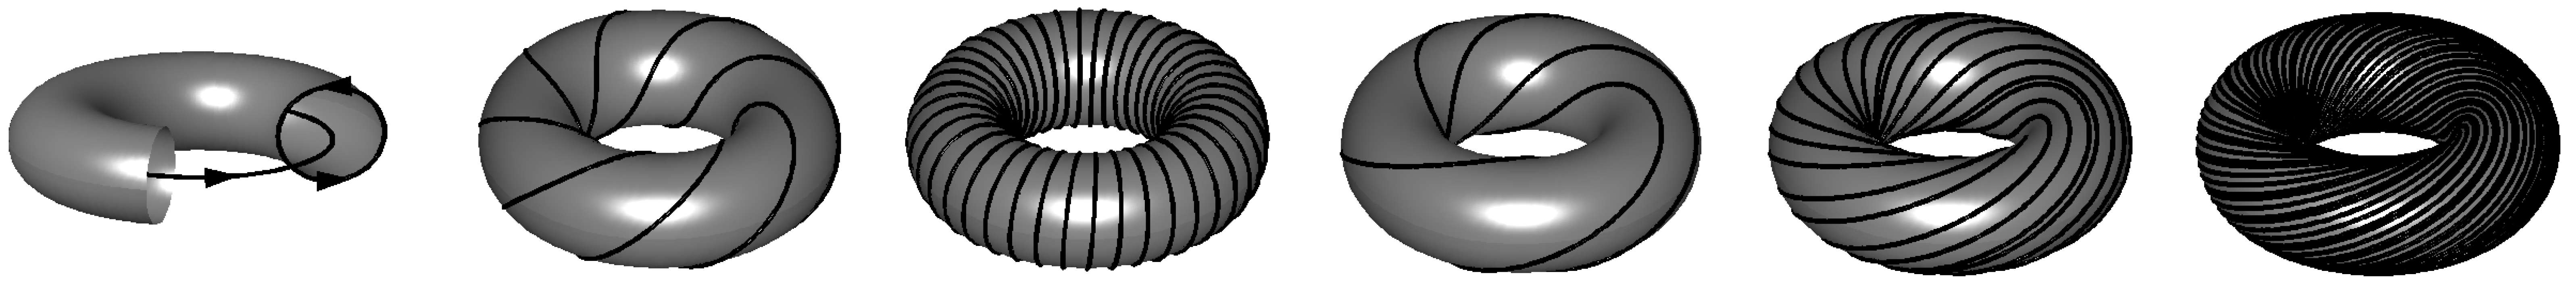
\includegraphics[width=\linewidth]{paqp.png}
	\caption{a) Flow on the surface of a torus can be described by a superposition of movements along two circles, one inside the torus and one around it.\\b) Here $\omega_i:\omega_a=8:3$.\\c) Here $\omega_i:\omega_a=1:40$.\\d) e) f) Here $\omega_i:\omega_a=\sqrt{2}$.}
	\label{fig:paqp}
\end{figure}
\subsection{Lorenz System}{\label{sec:ls}}
\paragraph{The Lorenz Equations}
In 1963, the MIT meteorologist Edward Lorenz constructed a highly simplified model of a convecting fluid.
This simple model also displays a wide variety of behavior and for some parameter values is chaotic.
\begin{equation}{\label{eq:ls}}
	\begin{aligned}
		\dot{x}&=\sigma(y-x)\\
		\dot{y}&=rx-y-xz\quad\text{with}\quad r,b,\sigma\geq0\\
		\dot{z}&=xy-bz
	\end{aligned}
\end{equation}
here $x$ measures the rate of convective overturning, $y$ measures the horizontal temperature variation, $z$ measures the vertical temperature variation, $\sigma$ is the \emph{Prandtl number}, $r$ is the \emph{Rayleigh number}, and $b$ is a scaling factor.
The Prandtl number is related to the fluid viscosity, and the Rayleigh number is related to the temperature difference between the top and bottom of the column.
Lorenz studied the system when $\sigma=10$ and $b=\frac{8}{3}$.\\
\subsubsection{Properties of Lorenz System}
\begin{itemize}
	\item System (\ref{eq:ls}) has natural symmetry $(x, y, z)\rightarrow(-x,-y, z)$.
	\item The $z-$axis is invariant.
	\item The flow is volume contracting since $\nabla\cdot\mathbf{x}=-(\sigma+b+1)<0$, where $\mathbf{x}$ is the vector field.
	\item The Lorenz system (\ref{eq:ls}) has the fixed points
	\begin{equation}{\label{eq:sls}}
		\mathbf{\tilde{x}}_1=
		\begin{pmatrix}
			0\\0\\0
		\end{pmatrix}\quad\text{and}\quad
		\mathbf{\tilde{x}}_{2,3}=
		\begin{pmatrix}
			\pm\sqrt{b(r-1)}\\[5pt]
			\pm\sqrt{b(r-1)}\\[5pt]
			r-1
		\end{pmatrix}\quad\text{if}\quad r\geq1
	\end{equation}
	As before, the stability of the fixed points is determined by the Jacobian matrix $J(x)$, which is given explicitly for the general three-dimensional case and $J_L(x)$ for the Lorenz system by
	\begin{equation}
		J(\mathbf{x})=
		\begin{pmatrix}
			\dfrac{\partial\dot{x}}{\partial x}&\dfrac{\partial\dot{x}}{\partial y}&\dfrac{\partial\dot{x}}{\partial z}\\[10pt]
			\dfrac{\partial\dot{y}}{\partial x}&\dfrac{\partial\dot{y}}{\partial y}&\dfrac{\partial\dot{y}}{\partial y}\\[10pt]
			\dfrac{\partial\dot{z}}{\partial x}&\dfrac{\partial\dot{z}}{\partial y}&\dfrac{\partial\dot{z}}{\partial z}
		\end{pmatrix}
		\quad\quad J_L(\mathbf{x})=
		\begin{pmatrix}
			-\sigma&\sigma&0\\
			r-z&-1&-x\\
			y&x&-b\\
		\end{pmatrix}
	\end{equation}
	The eigenvalues for origin is
	\begin{equation}
		\lambda_{1,2}=\frac{1}{2}\left\{-(\sigma+1)\pm\sqrt{(\sigma-1)^2+4\sigma r}\right\}\quad\text{and}\quad
		\lambda_3=-b
	\end{equation}
	\item At $r=1$ the system undergoes a bifurcation where two additional fixed points appear (Equation (\ref{eq:sls})).
	\begin{equation}
		r=0:
		\begin{cases}
			\lambda_1&=-1\\
			\lambda_2&=-\sigma\\
			\lambda_3&=-b
		\end{cases}\quad
		r=1:
		\begin{cases}
			\lambda_1&=0\\
			\lambda_2&=-\sigma-1\\
			\lambda_3&=-b
		\end{cases}\quad
		r>1:
		\begin{cases}
			\lambda_1&>0\\
			\lambda_2&<-\sigma-1\\
			\lambda_3&=-b
		\end{cases}
	\end{equation}
	The origin is stable for $0<r<1$ and unstable for $r>1$ where the two additional fixed points $\mathbf{\tilde{x}}_2$ and $\mathbf{\tilde{x}}_3$ exist and are stable for $1<r<r_H$.
	\item Instability points are characterized by a vanishing real part of the largest eigenvalue, $\Re\{\lambda\}=0$.
	Then, substitute $\lambda$ in (\ref{eq:ls23}) by $i\omega$ and after equating real and imaginary parts with zero, we get
	\begin{equation}{\label{eq:ls23}}
		\det[J(\mathbf{\tilde{x}}_{2,3})-\lambda I]=0\quad\rightarrow\quad
		\lambda^3+\lambda^2(\sigma+b+1)+\lambda b(\sigma+r)+2\sigma b(r-1)=0
	\end{equation}
	\begin{equation}
		\frac{2\sigma b(r-1)}{\sigma+b+1}=b(\sigma+r)\quad\text{with}\quad \sigma=10\quad b=\frac{8}{3}\quad\rightarrow\quad r_H\approx24.74
	\end{equation}
	\item At $r_H$ the two fixed points $\mathbf{\tilde{x}}_2$ and $\mathbf{\tilde{x}}_3$ undergo a Subcritical Hopf bifurcation.
	\item When $r>r_H$ a structure emerges, which belongs to a class of objects now called {\textbf{strange attractors}}, in this particular case the \emph{Lorenz attractor}. This is \emph{deterministic chaos}.
	Defined as: Aperiodic long-term behavior in a deterministic system that exhibits sensitive dependence on initial conditions\footnote{Here ‘aperiodic longterm behavior’ means that the trajectories do not settle down to a fixed point, or periodic or quasi-periodic orbit; ‘deterministic’ means that the system has no random input or parameters; and ‘sensitive dependence on initial conditions’ means that nearby trajectories may separate exponentially fast.}.
	\item At $r\approx13.926$, there is a homoclinic bifurcation and the system enters a state of transient chaos.
	\item At $r\approx24.06$, a strange attractor is formed.
\end{itemize}
\begin{comment}
	\begin{figure}[h!]
	\centering
	\begin{subfigure}{0.45\linewidth}
	\centering
	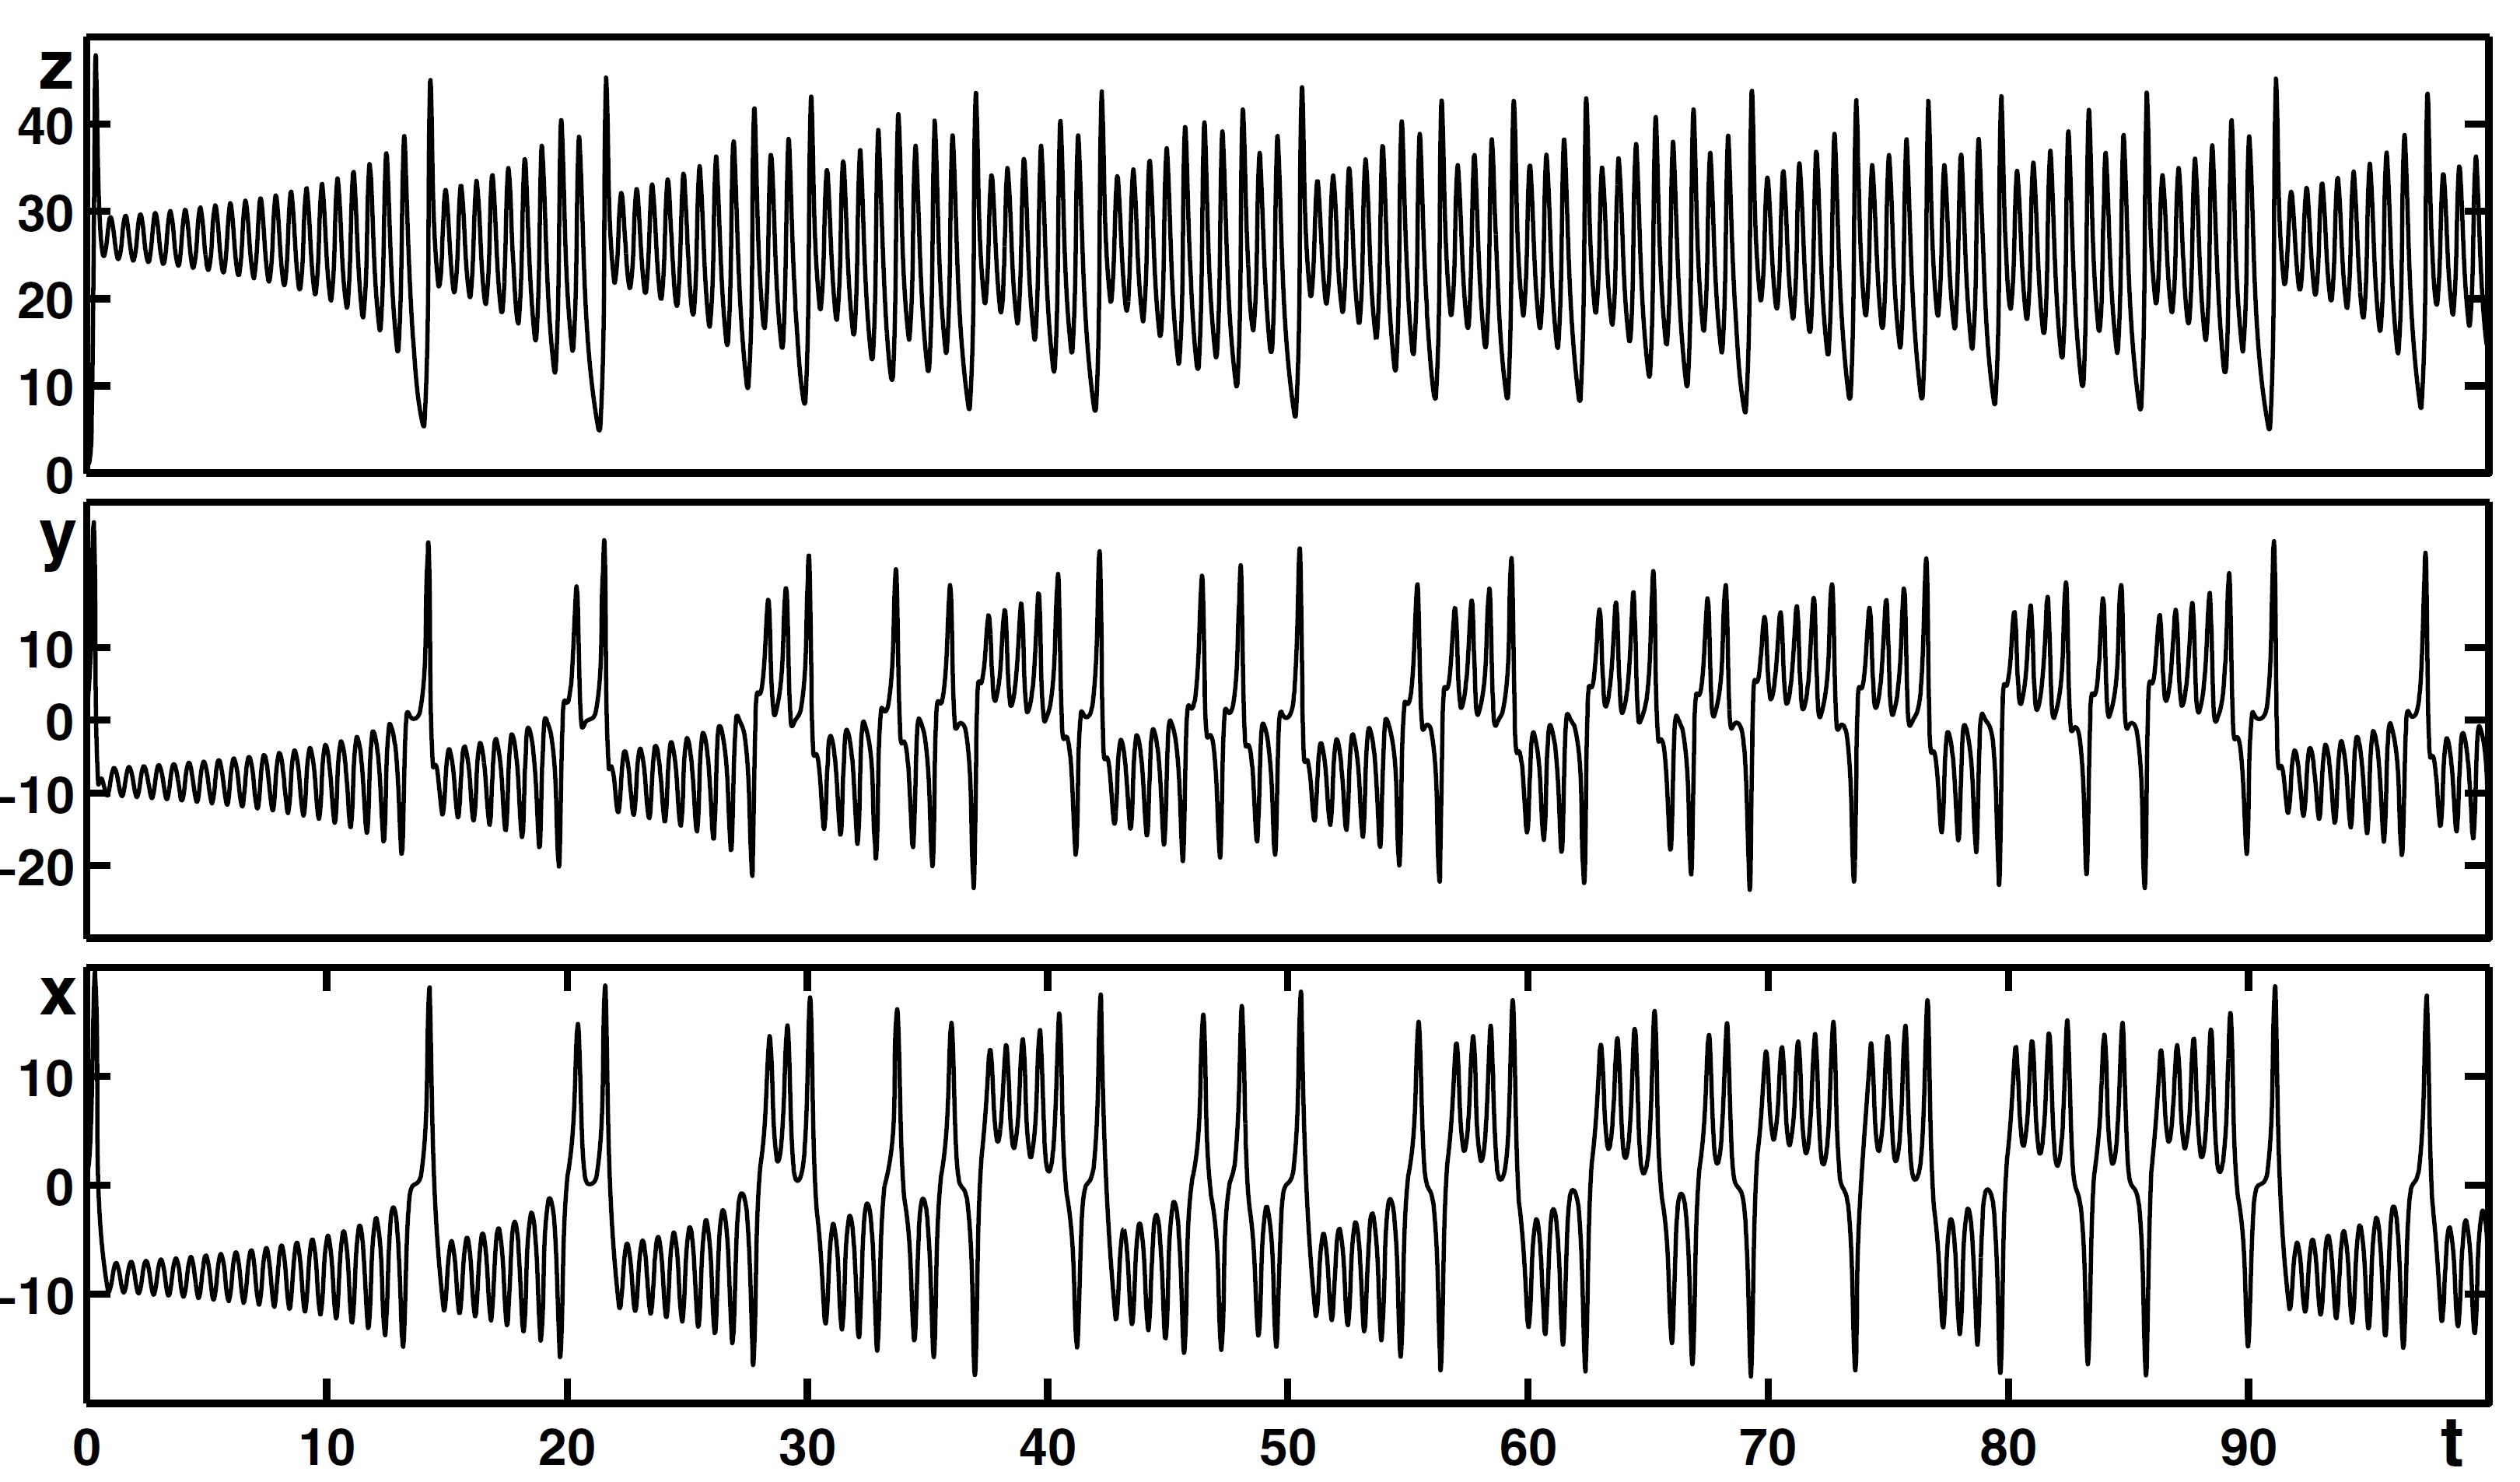
\includegraphics[width=\linewidth]{tsls.png}
	\caption{Time series for the Lorenz system for $\sigma=10, b=\frac{8}{3}$ and $r=28$.}
	\label{fig:tsls}
	\end{subfigure}
	\vline
	\begin{subfigure}{0.45\linewidth}
	\centering
	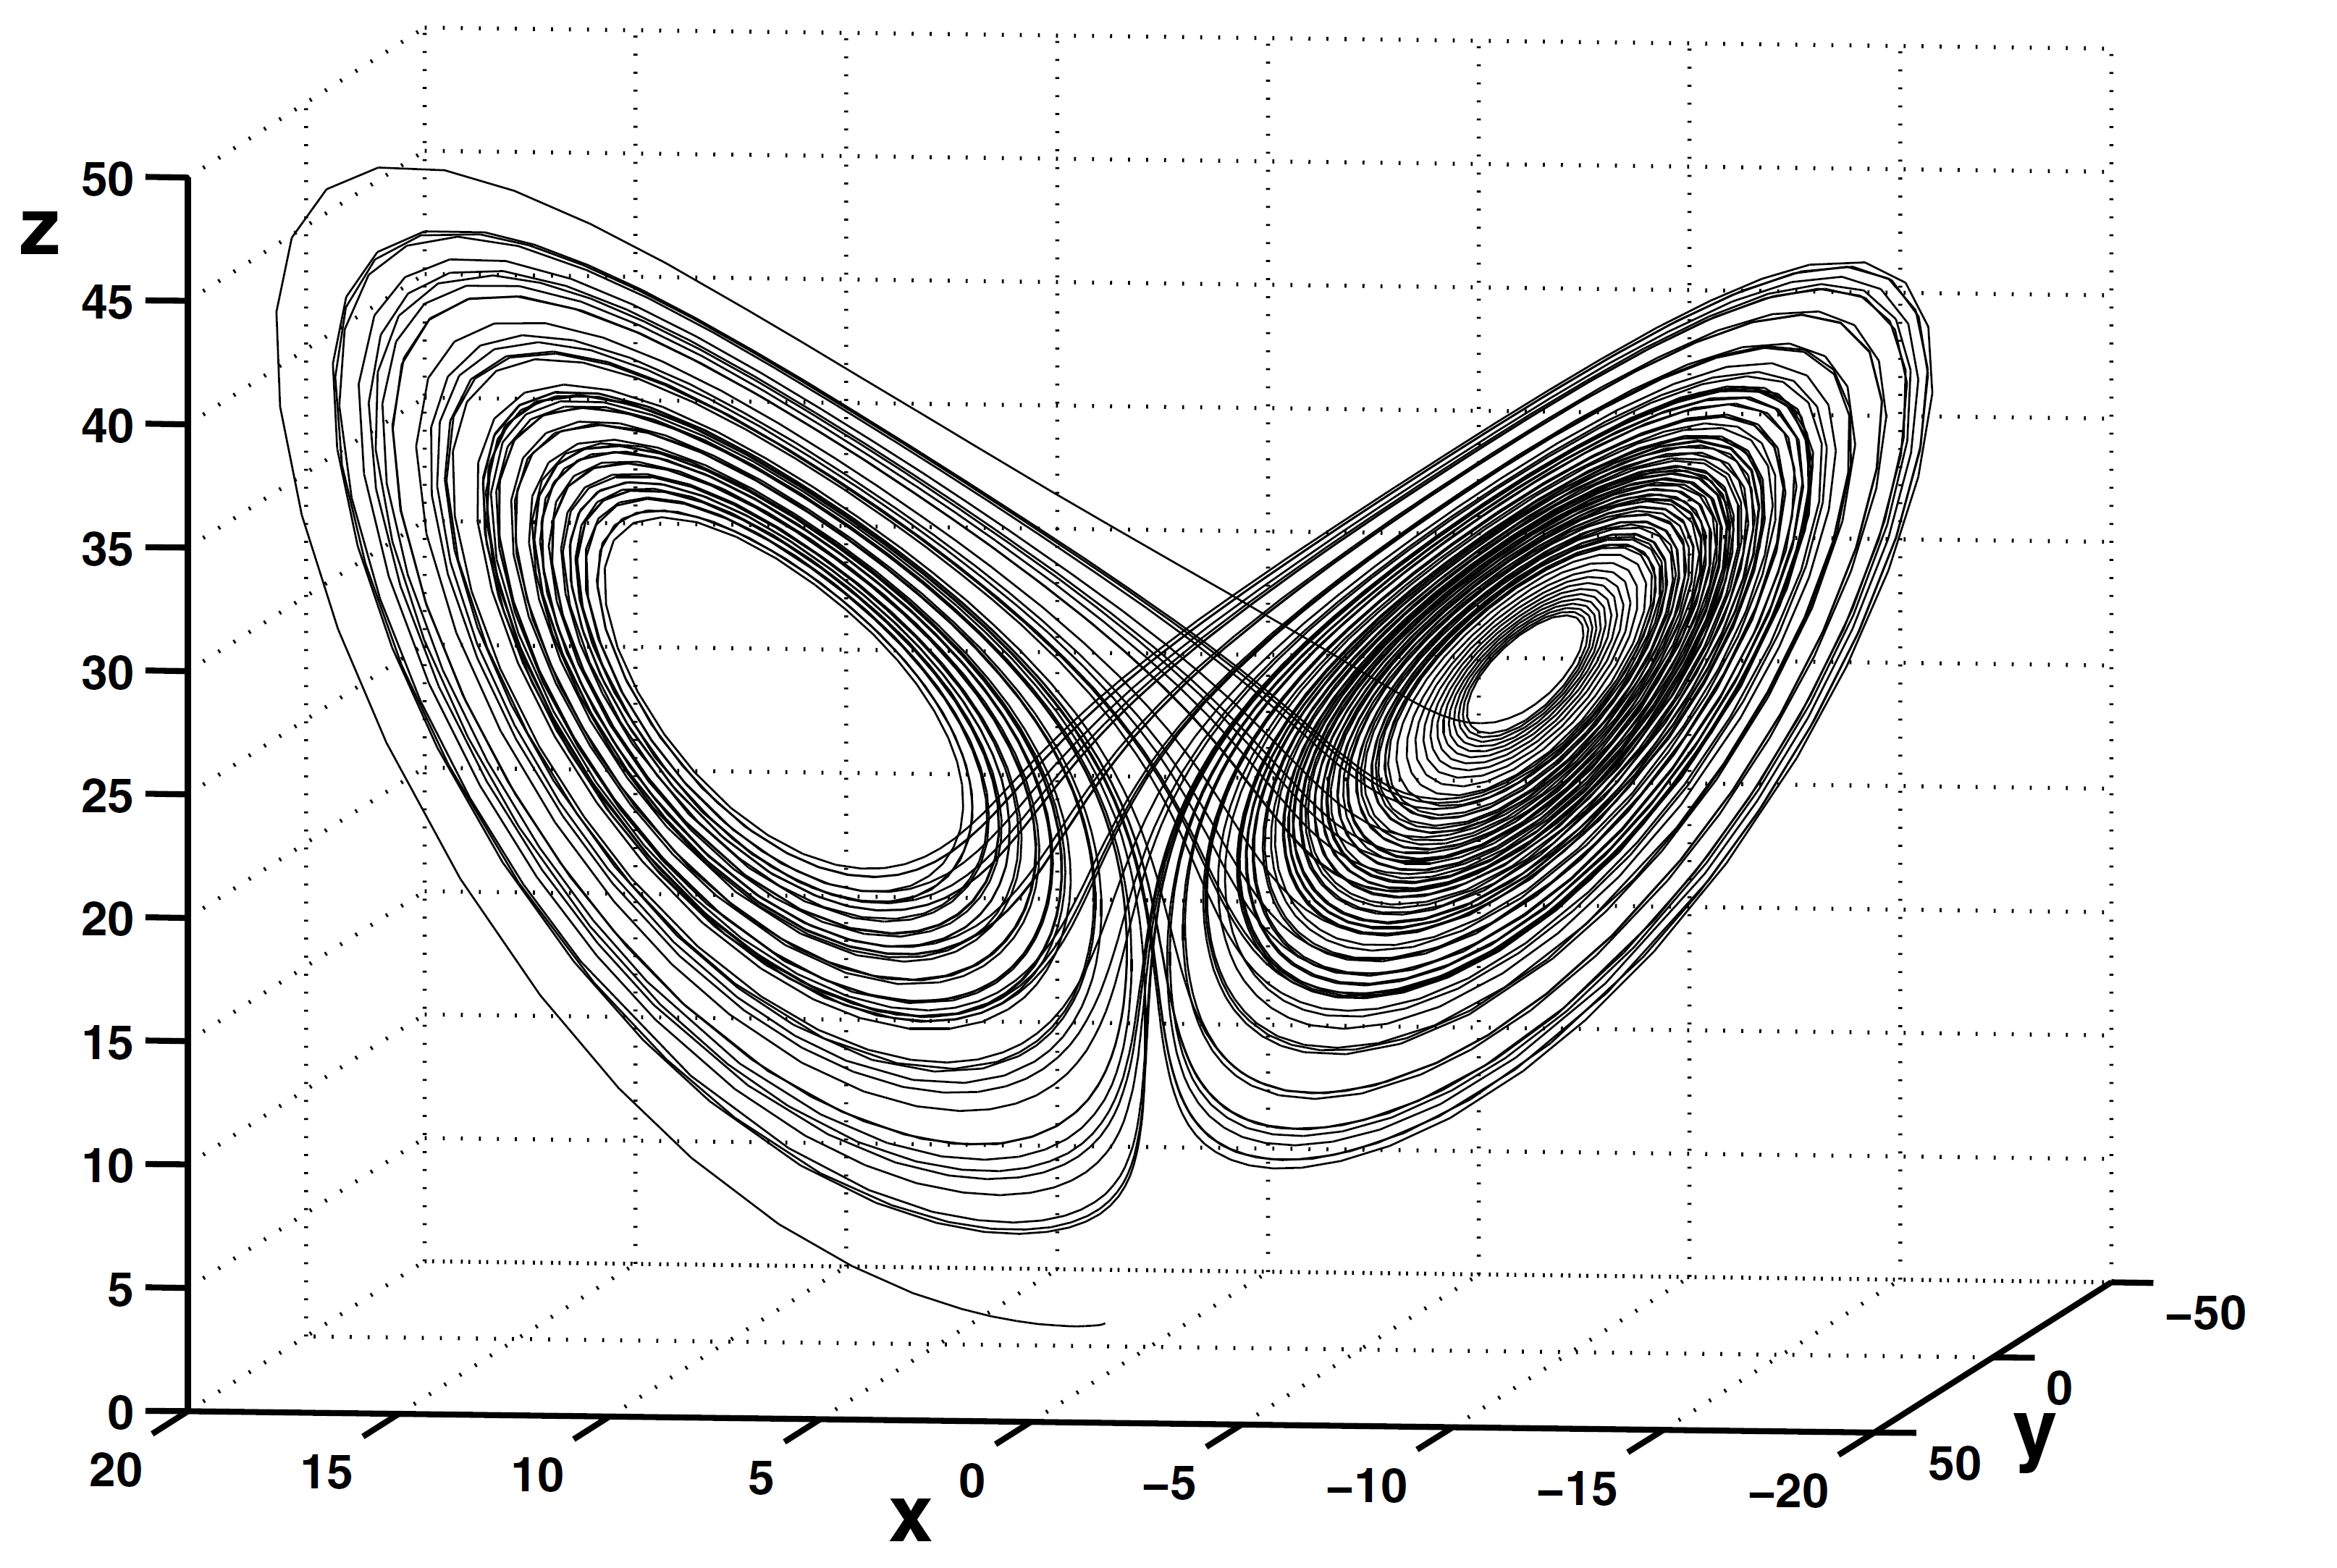
\includegraphics[width=\linewidth]{lals.png}
	\caption{The Lorenz attractor as a three-dimensional plot of the time series (Figure (\ref{fig:tsls}))}
	\label{fig:lals}
	\end{subfigure}
	\end{figure}
\end{comment}
The Lorenz attractor consists of two sheets roughly defined by planes for positive and negative values of $x$ where the trajectory spirals outwards with the fixed points $\mathbf{\tilde{x}}_{2,3}$ located at the centers of these spirals.
\begin{figure}[h!]
	\centering
	\begin{subfigure}{0.45\linewidth}
		\centering
		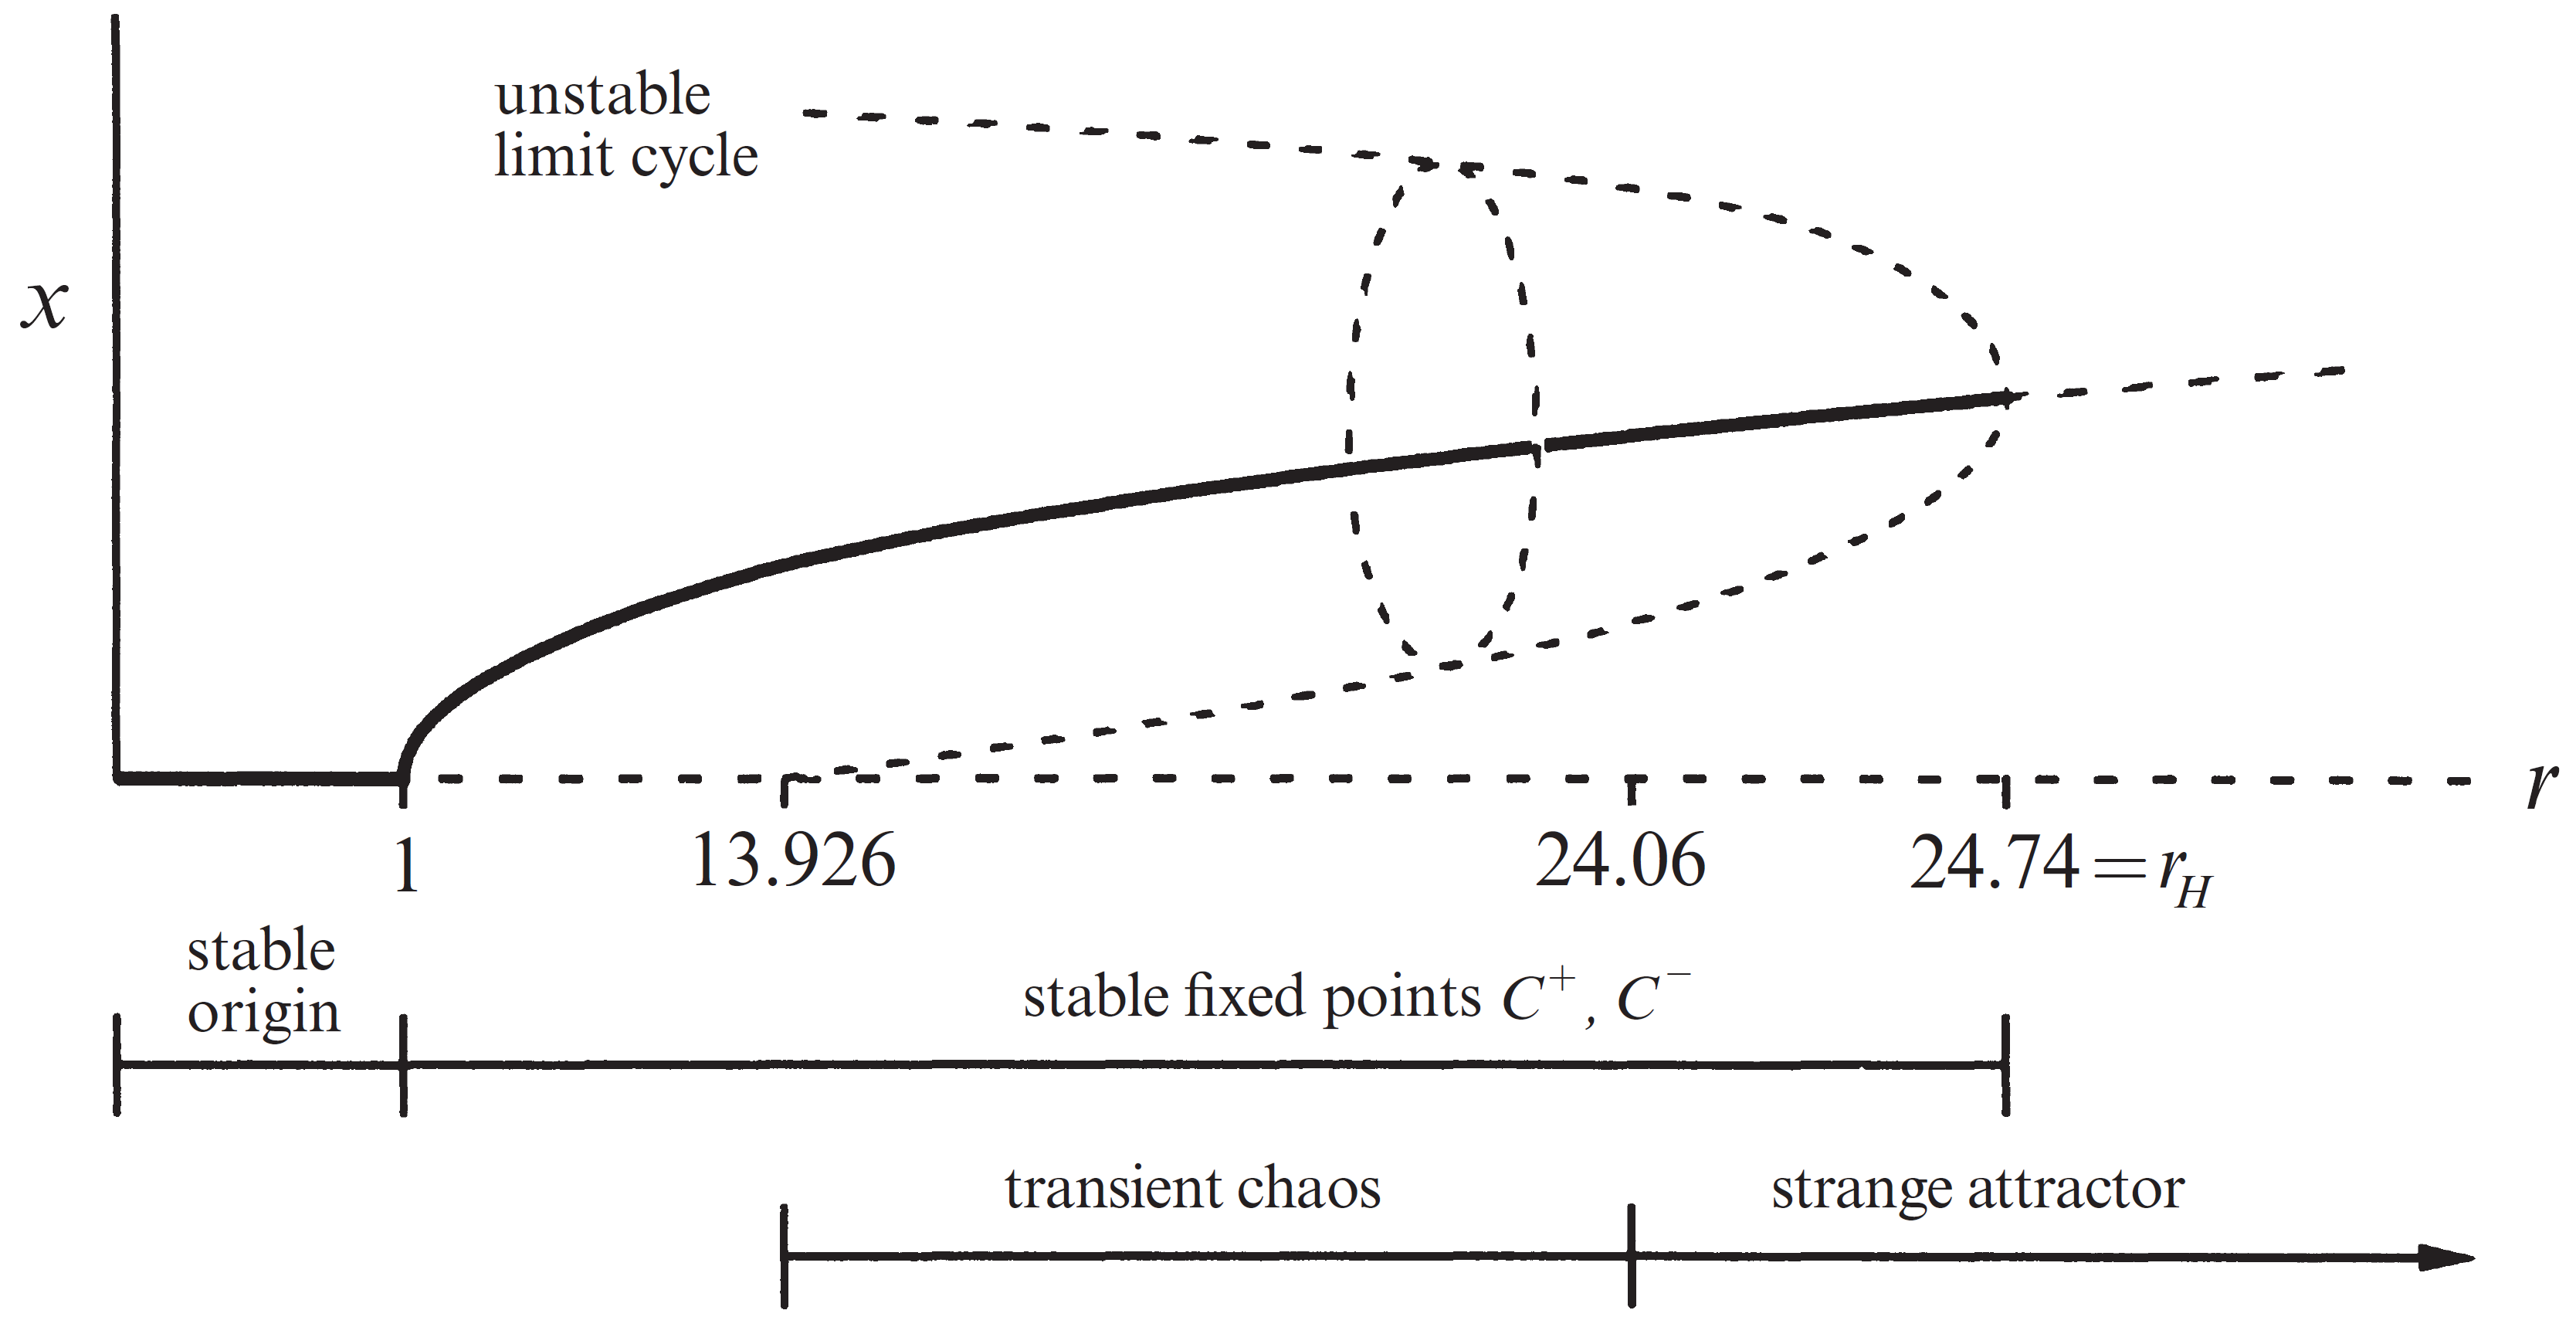
\includegraphics[width=\linewidth]{bfls.png}
		\caption{Parameter Space of Lorenz System}
		\label{fig:bfls}
	\end{subfigure}
	\vline
	\begin{subfigure}{0.45\linewidth}
		\centering
		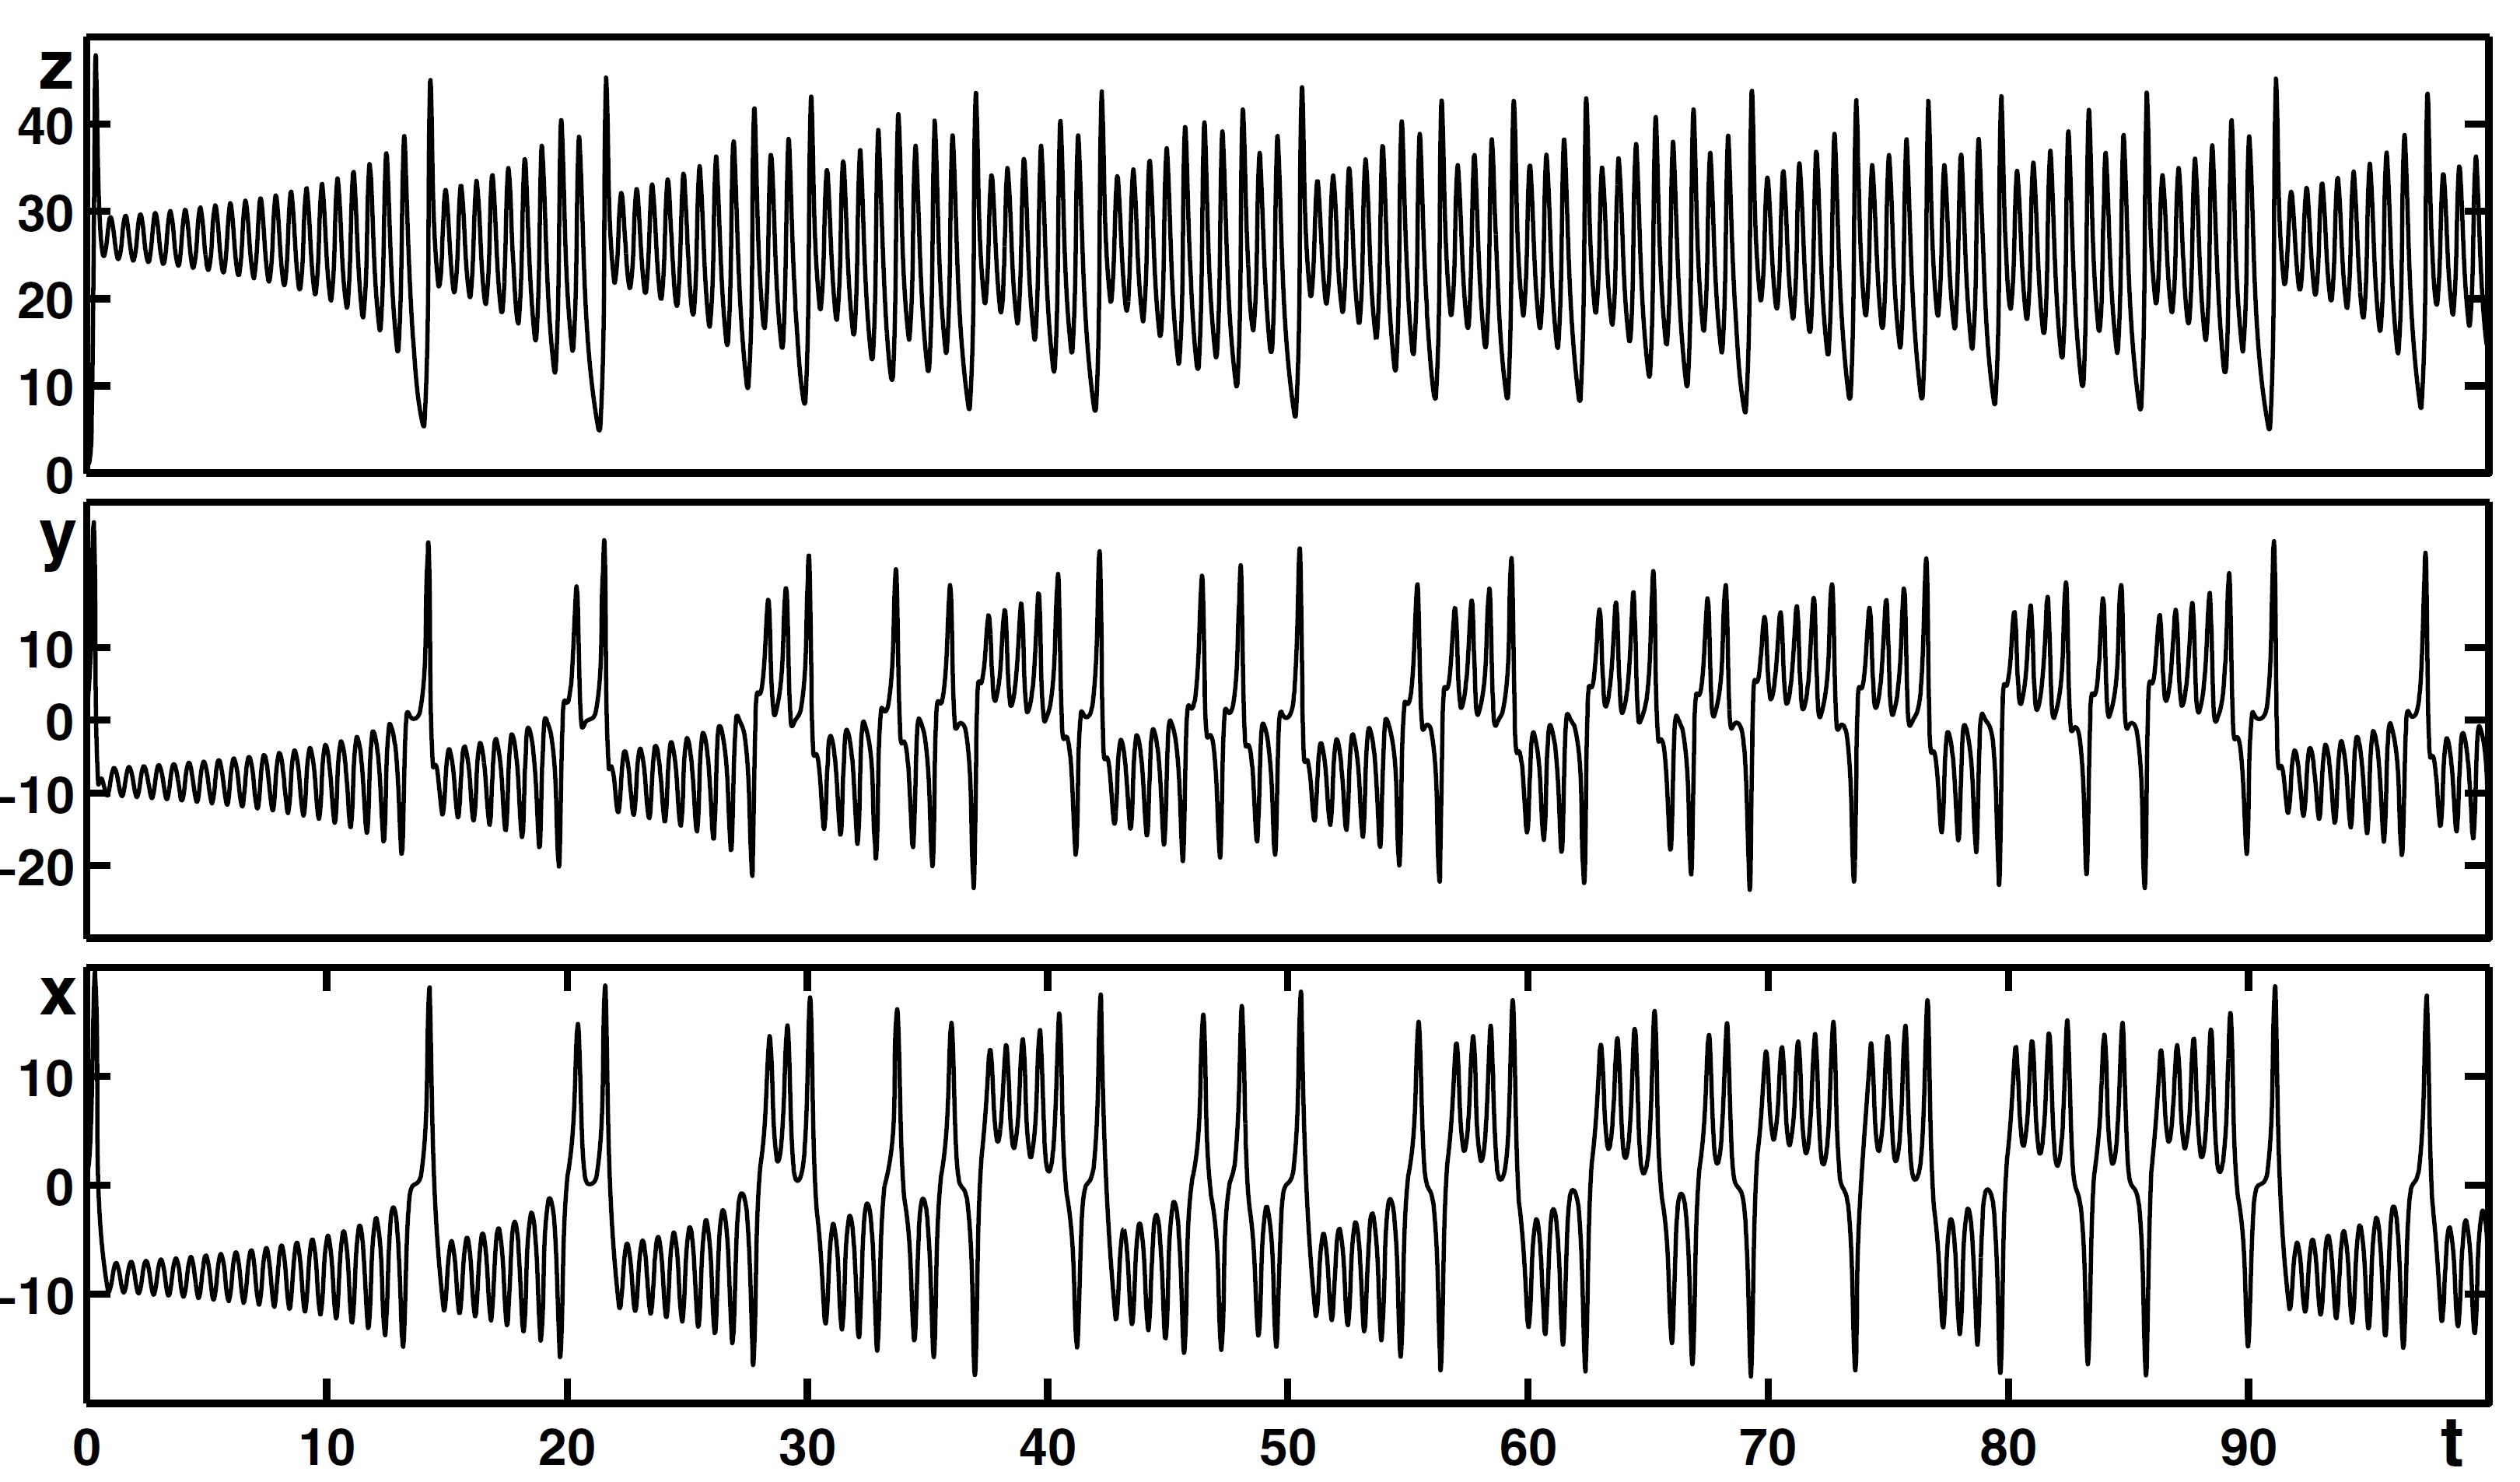
\includegraphics[width=\linewidth]{tsls.png}
		\caption{Time series for the Lorenz system for $\sigma=10, b=\frac{8}{3}$ and $r=28$.}
		\label{fig:tsls}
	\end{subfigure}
\end{figure}
\begin{figure}[h!]
	\centering
	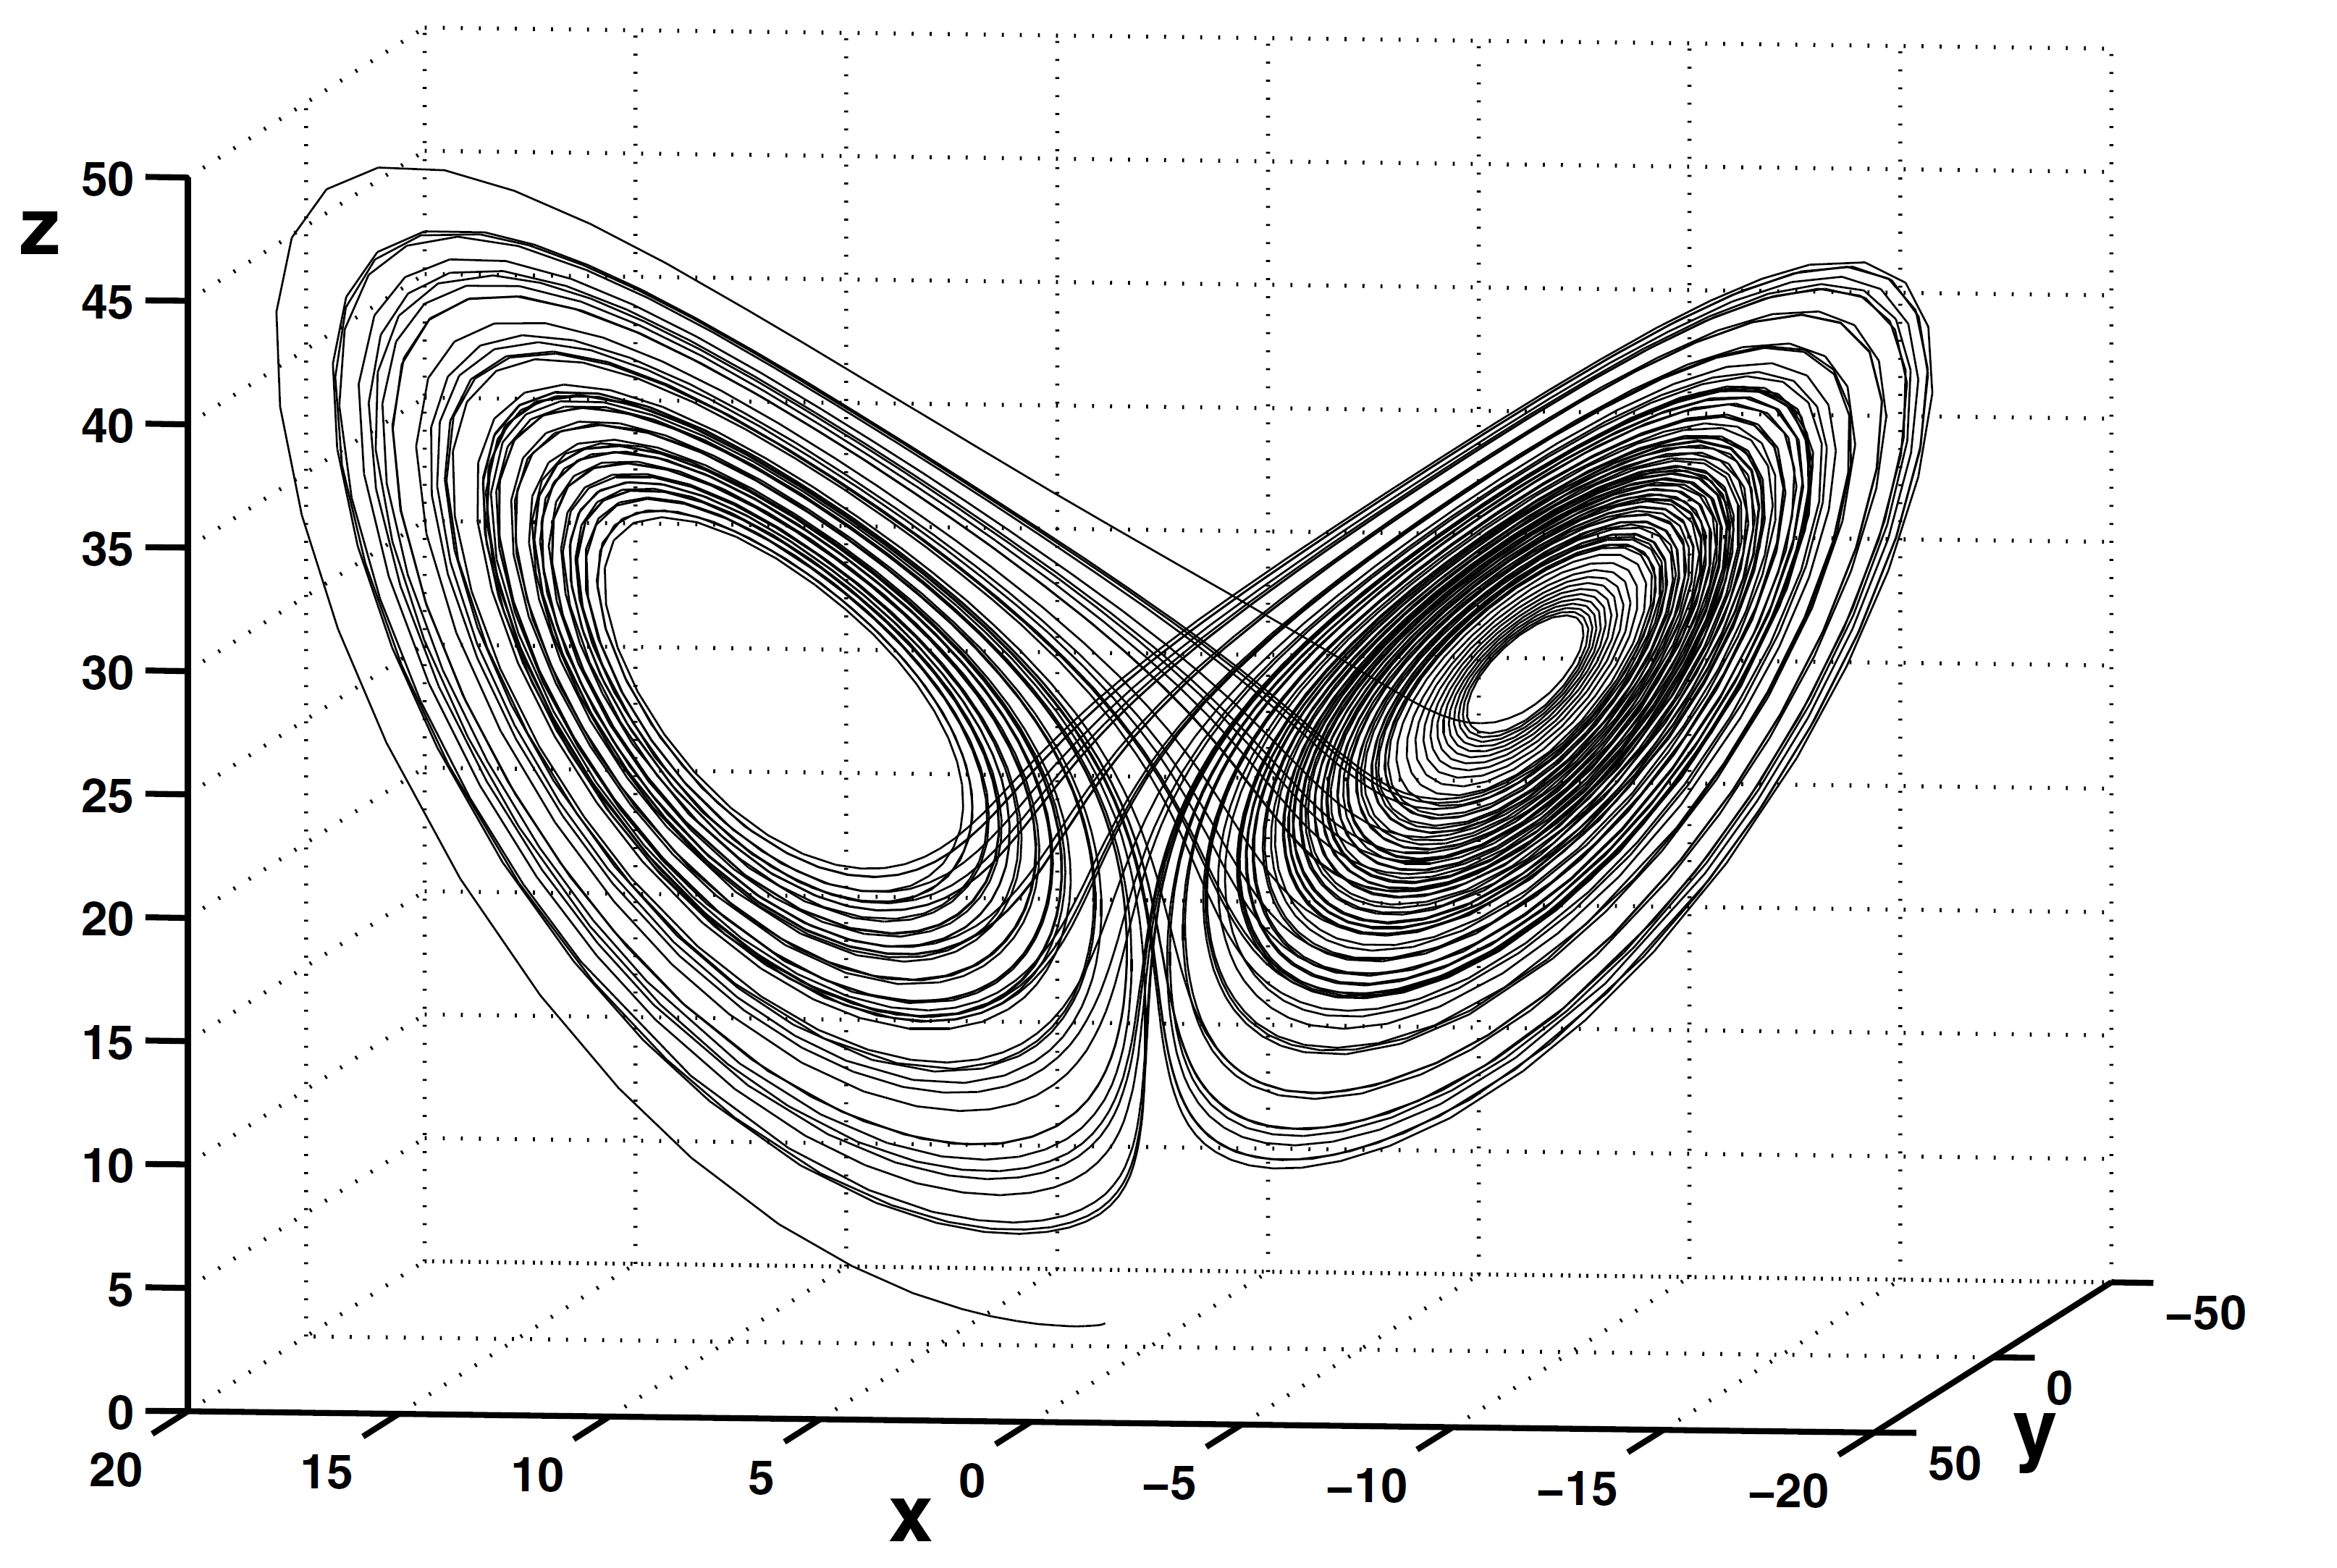
\includegraphics[width=0.7\linewidth]{lals.png}
	\caption{The Lorenz attractor as a three-dimensional plot of the time series (Figure (\ref{fig:tsls}))}
	\label{fig:lals}
\end{figure}
\subsubsection{Properties of Strange Attractor}
\begin{itemize}
	\item The trajectory is aperiodic.
	\item The trajectory remains on the attractor forever. (the attractor is \emph{invariant})
	\item The general form is independent of initial conditions.
	\item The sequence of windings is sensitive to initial conditions.
	\item The attractor has fractal structure.
\end{itemize}
\subsection{R\"ossler System}{\label{sec:rs}}
The R\"ossler system with its standard parameters for chaotic behavior is given by
\begin{equation}
	\begin{aligned}
		\dot{x}&=-y-z\\
		\dot{y}&=x+ay\\
		\dot{z}&=b+z(x-c)
	\end{aligned}\quad\text{with}\quad
	a=b=0.2
\end{equation}
The dynamics of the R\"ossler system consist of a spiral movement in the $xy-$plane and escapes along the positive $z-$direction.
A three-dimensional plot of the R\"ossler attractor together with the time series for the $x-, y-$ and $z-$coordinates are shown in Figure (\ref{fig:rars}).
For $a=b=0.2$ kept fixed and varying $c$ the R\"ossler system undergoes a sequence of period doublings from a simple limit cycle at $c =2.5$ to a strange attractor at $c = 5$.
Beyond this first chaotic r\`egime there are again limit cycles that bifurcate into orbits of increasing complexity, before the standard attractor at $c=5.7$ is reached.
\begin{figure}[h!]
	\centering
	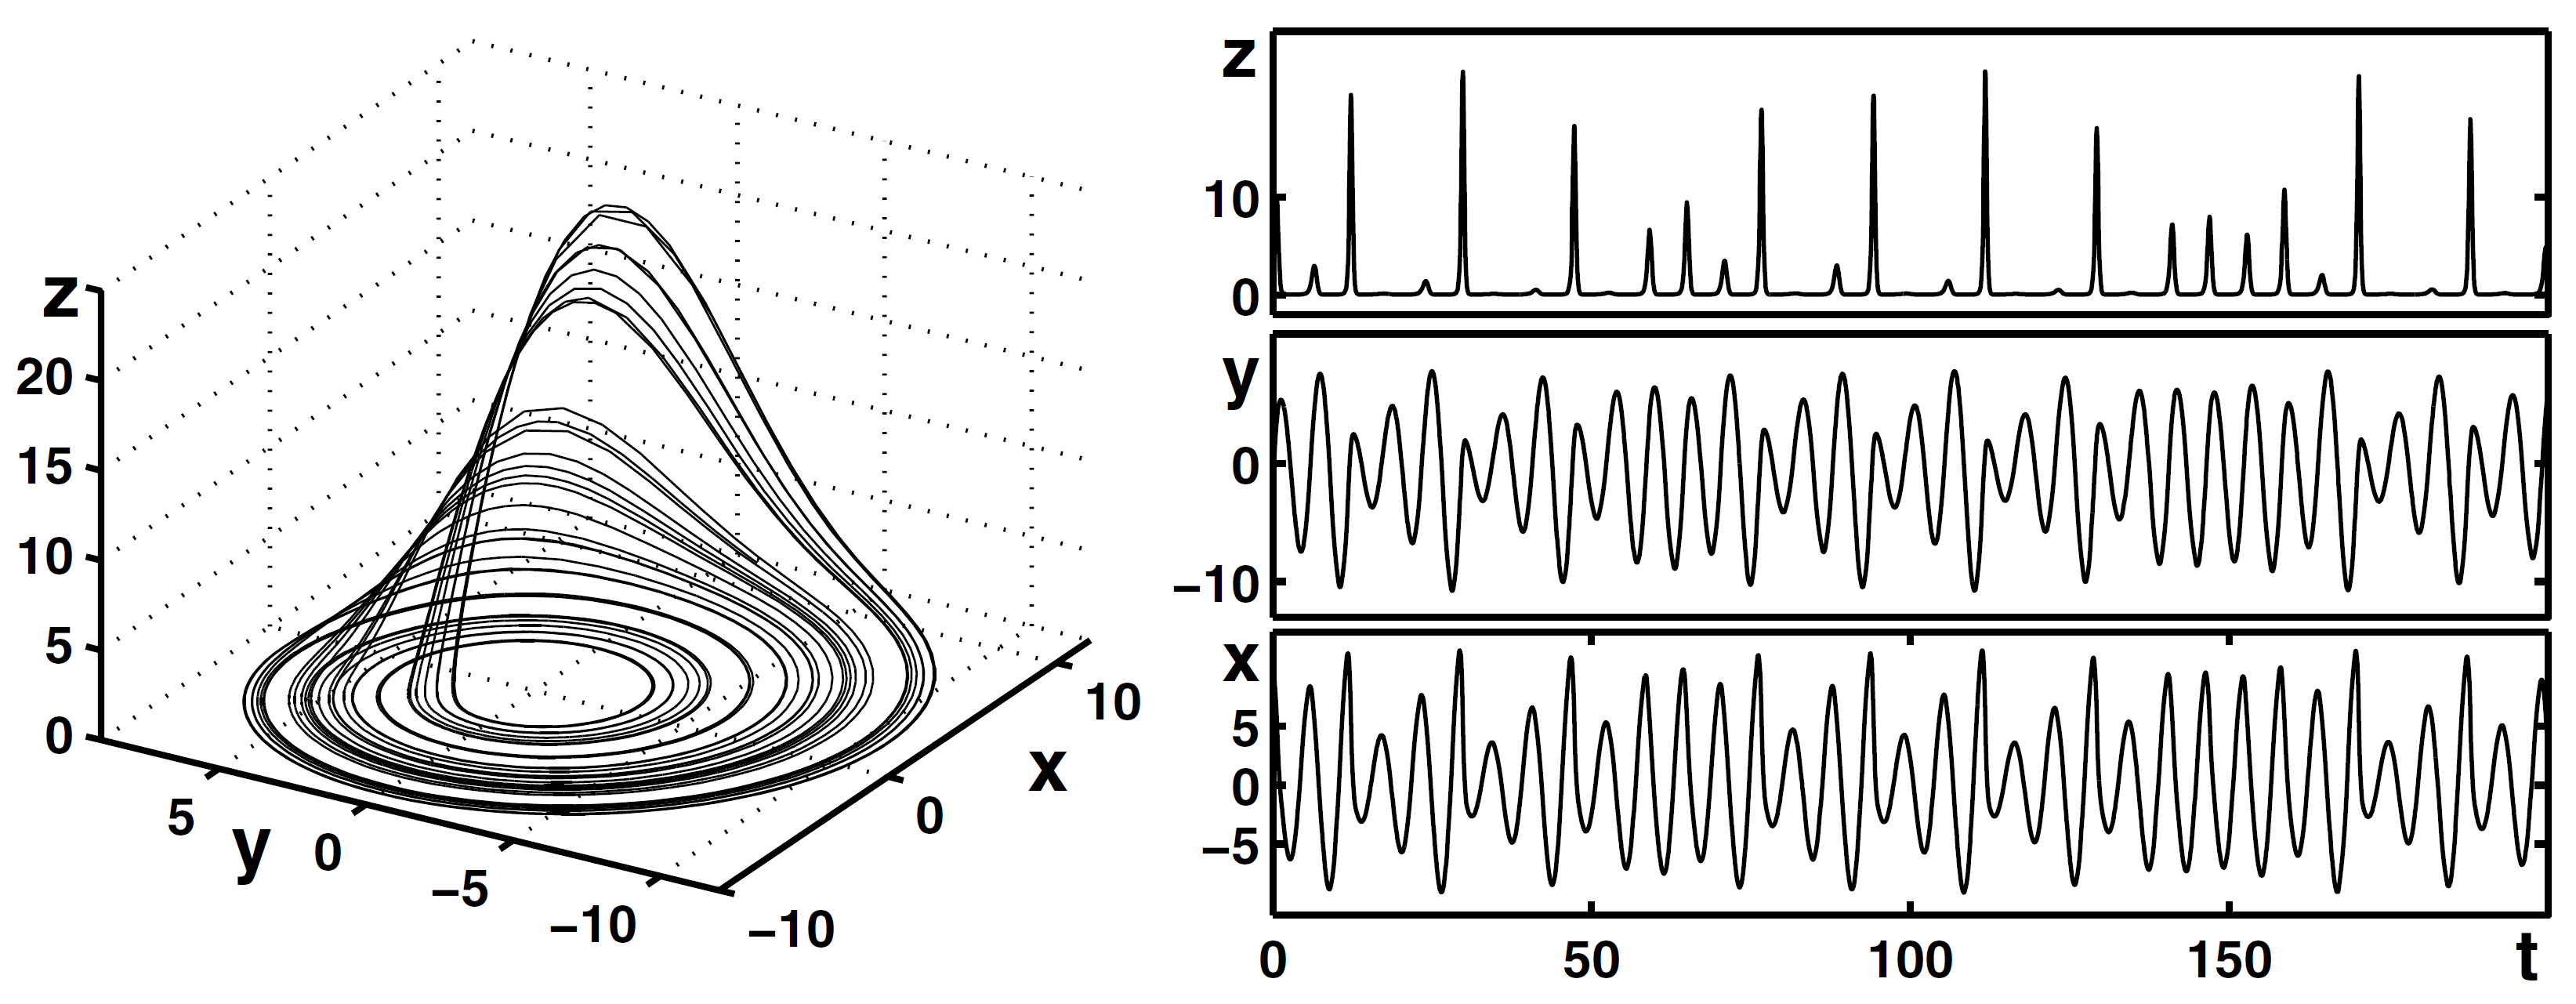
\includegraphics[width=\linewidth]{rars.png}
	\caption{The R\"ossler attractor in a three-dimensional plot (left) and time series of the corresponding $x-, y-$ and $z-$coordinates (right).\\Parameters: $a=b=0.2, c =5.7$.}
	\label{fig:rars}
\end{figure}